\section{Độ phức tạp của bài toán tìm kiếm trong Cờ vua}

Cờ vua không chỉ là một trò chơi, mà còn là một bài toán thử thách giới hạn tính toán của máy tính. Điểm mấu chốt nằm ở \textbf{số Shannon} ($10^{120}$), một con số ước tính tổng số trạng thái có thể xảy ra trong một ván cờ. Để so sánh, số lượng nguyên tử trong vũ trụ quan sát được chỉ vào khoảng $10^{80}$.

\begin{figure}[H]
    \centering
    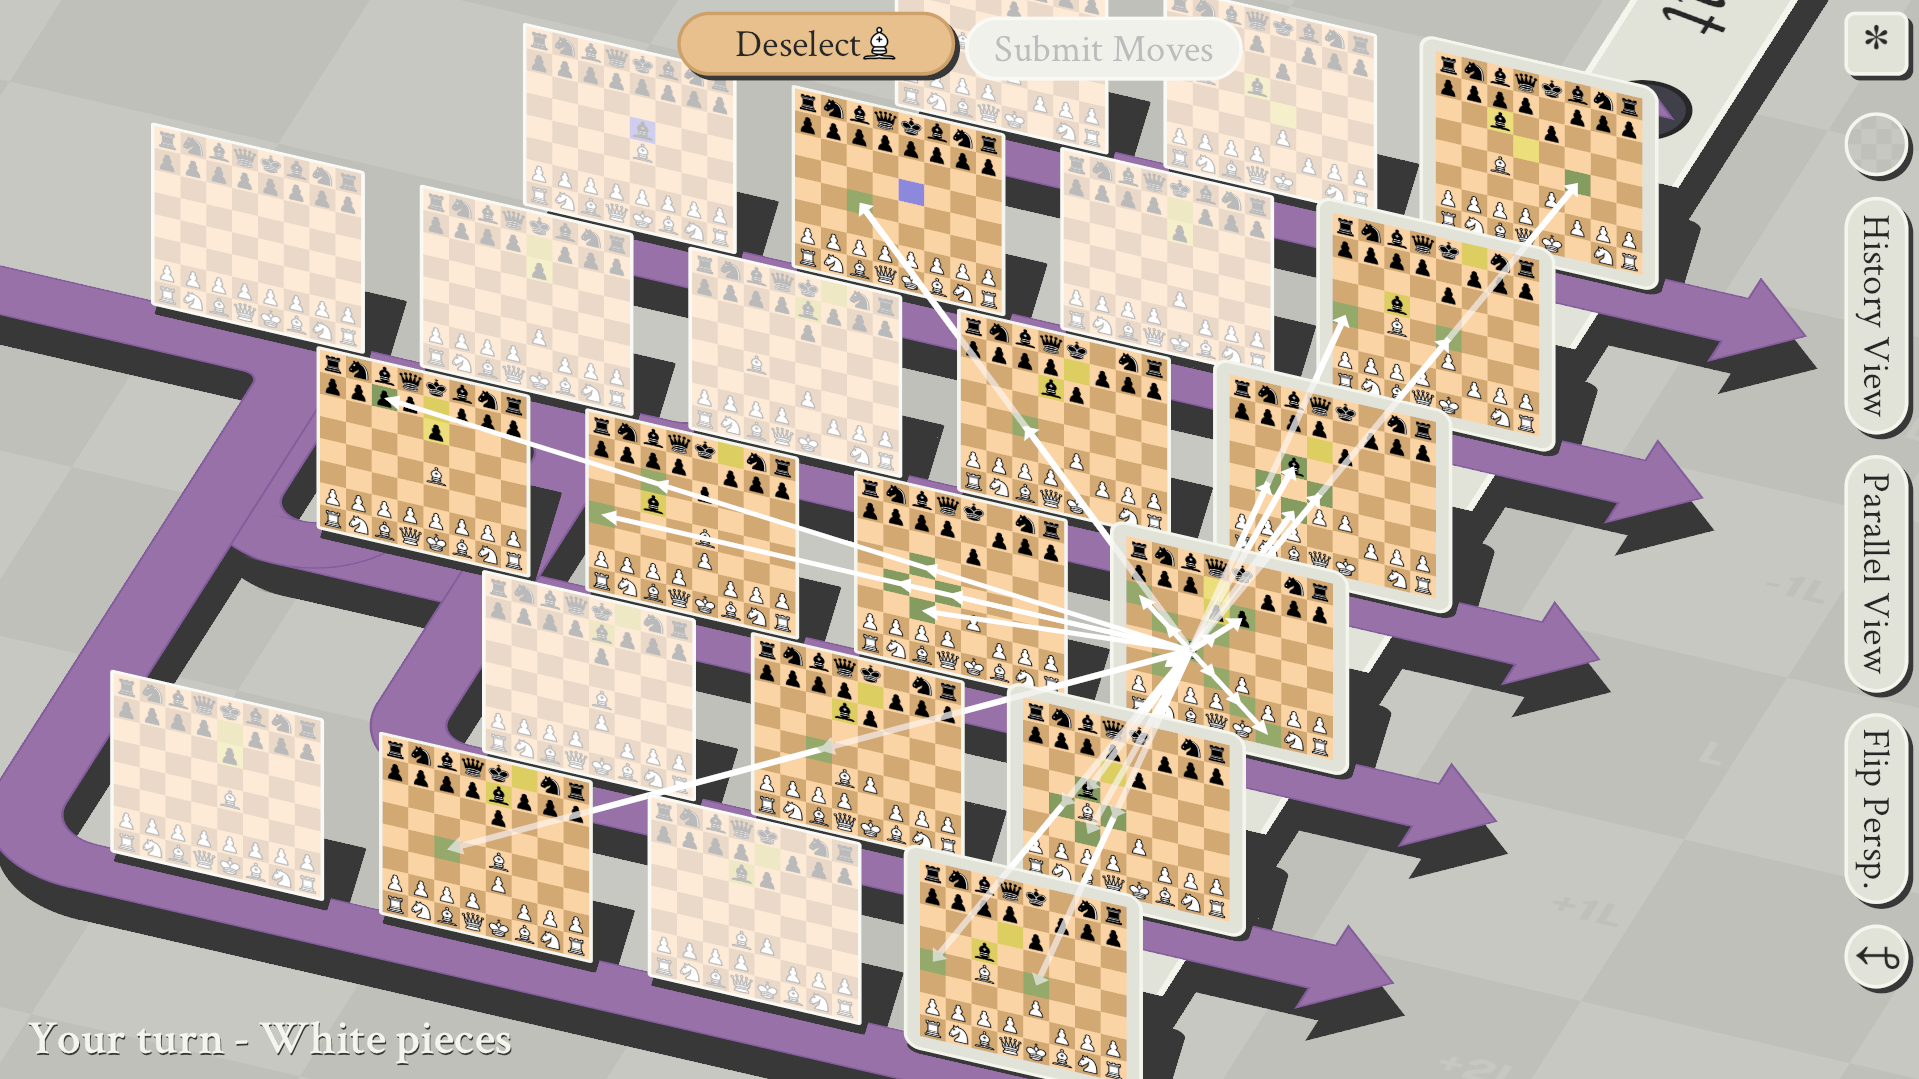
\includegraphics[width=0.7\linewidth]{../../images/ai/space-complex.png}
    \caption{Minh họa sự phức tạp và các trạng thái liên kết trong cây trò chơi}
\end{figure}

Nếu một máy tính có thể duyệt được 1 triệu nước đi mỗi giây, nó sẽ mất hàng tỷ tỷ năm để duyệt hết toàn bộ cây trò chơi. Do đó, việc sử dụng các thuật toán "vét cạn" (Brute-force) là hoàn toàn bất khả thi. Điều này thúc đẩy việc nghiên cứu các thuật toán có khả năng:
\begin{itemize}
    \item \textbf{Cắt tỉa không gian tìm kiếm:} Loại bỏ sớm các nhánh không mang lại kết quả tốt.
    \item \textbf{Ước lượng thế trận:} Sử dụng các hàm đánh giá thông minh để thay thế việc phải duyệt đến tận cùng ván đấu.
\end{itemize}

\section{Sức mạnh của Alpha-Beta Pruning và tri thức con người}

Thuật toán Alpha-Beta Pruning là một bước tiến quan trọng từ Minimax. Động lực chính khi áp dụng thuật toán này trong dự án là khả năng tích hợp \textbf{tri thức con người} vào máy tính thông qua các hàm đánh giá (Heuristic).

\begin{figure}[H]
    \centering
    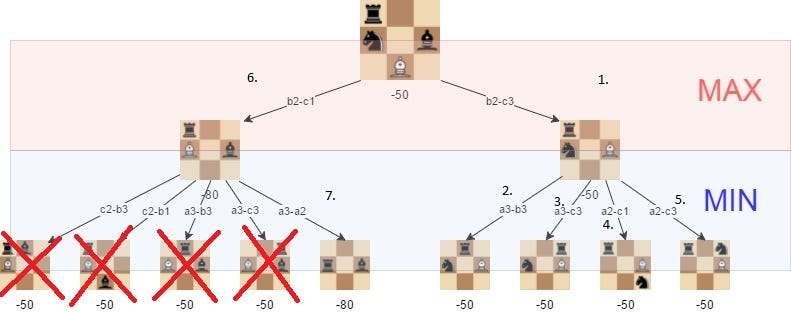
\includegraphics[width=0.8\linewidth]{../../images/ai/alphabeta-visual.jpg}
    \caption{Cơ chế duyệt sâu (DFS) và cắt tỉa các nhánh vô ích trong Alpha-Beta}
\end{figure}

Bằng cách duy trì hai giá trị Alpha (mức tối ưu cho người chơi MAX) và Beta (mức tối ưu cho người chơi MIN), thuật toán cho phép máy tính bỏ qua những nước đi chắc chắn tệ hơn các nước đi đã tìm thấy trước đó. Việc nghiên cứu Alpha-Beta giúp chúng ta hiểu cách:
\begin{itemize}
    \item Lượng hóa giá trị của quân cờ (Quân Hậu mạnh hơn quân Tốt bao nhiêu lần?).
    \item Đánh giá vị trí chiến thuật (Tại sao quân Mã ở trung tâm lại mạnh hơn ở góc?).
\end{itemize}

\section{Tiềm năng của Monte Carlo Tree Search (MCTS)}

Nếu Alpha-Beta dựa trên "logic và tri thức", thì MCTS lại dựa trên "trải nghiệm và thống kê". Động lực thực hiện MCTS bắt nguồn từ sự thành công của AlphaGo, khi AI có thể đánh bại con người trong các trò chơi có không gian trạng thái cực lớn mà không cần quá nhiều hàm đánh giá thủ công.

\begin{figure}[H]
    \centering
    % Giả sử bạn sẽ thêm ảnh mcts_process.png sau, hiện tại dùng logo hoặc ảnh state làm placeholder
    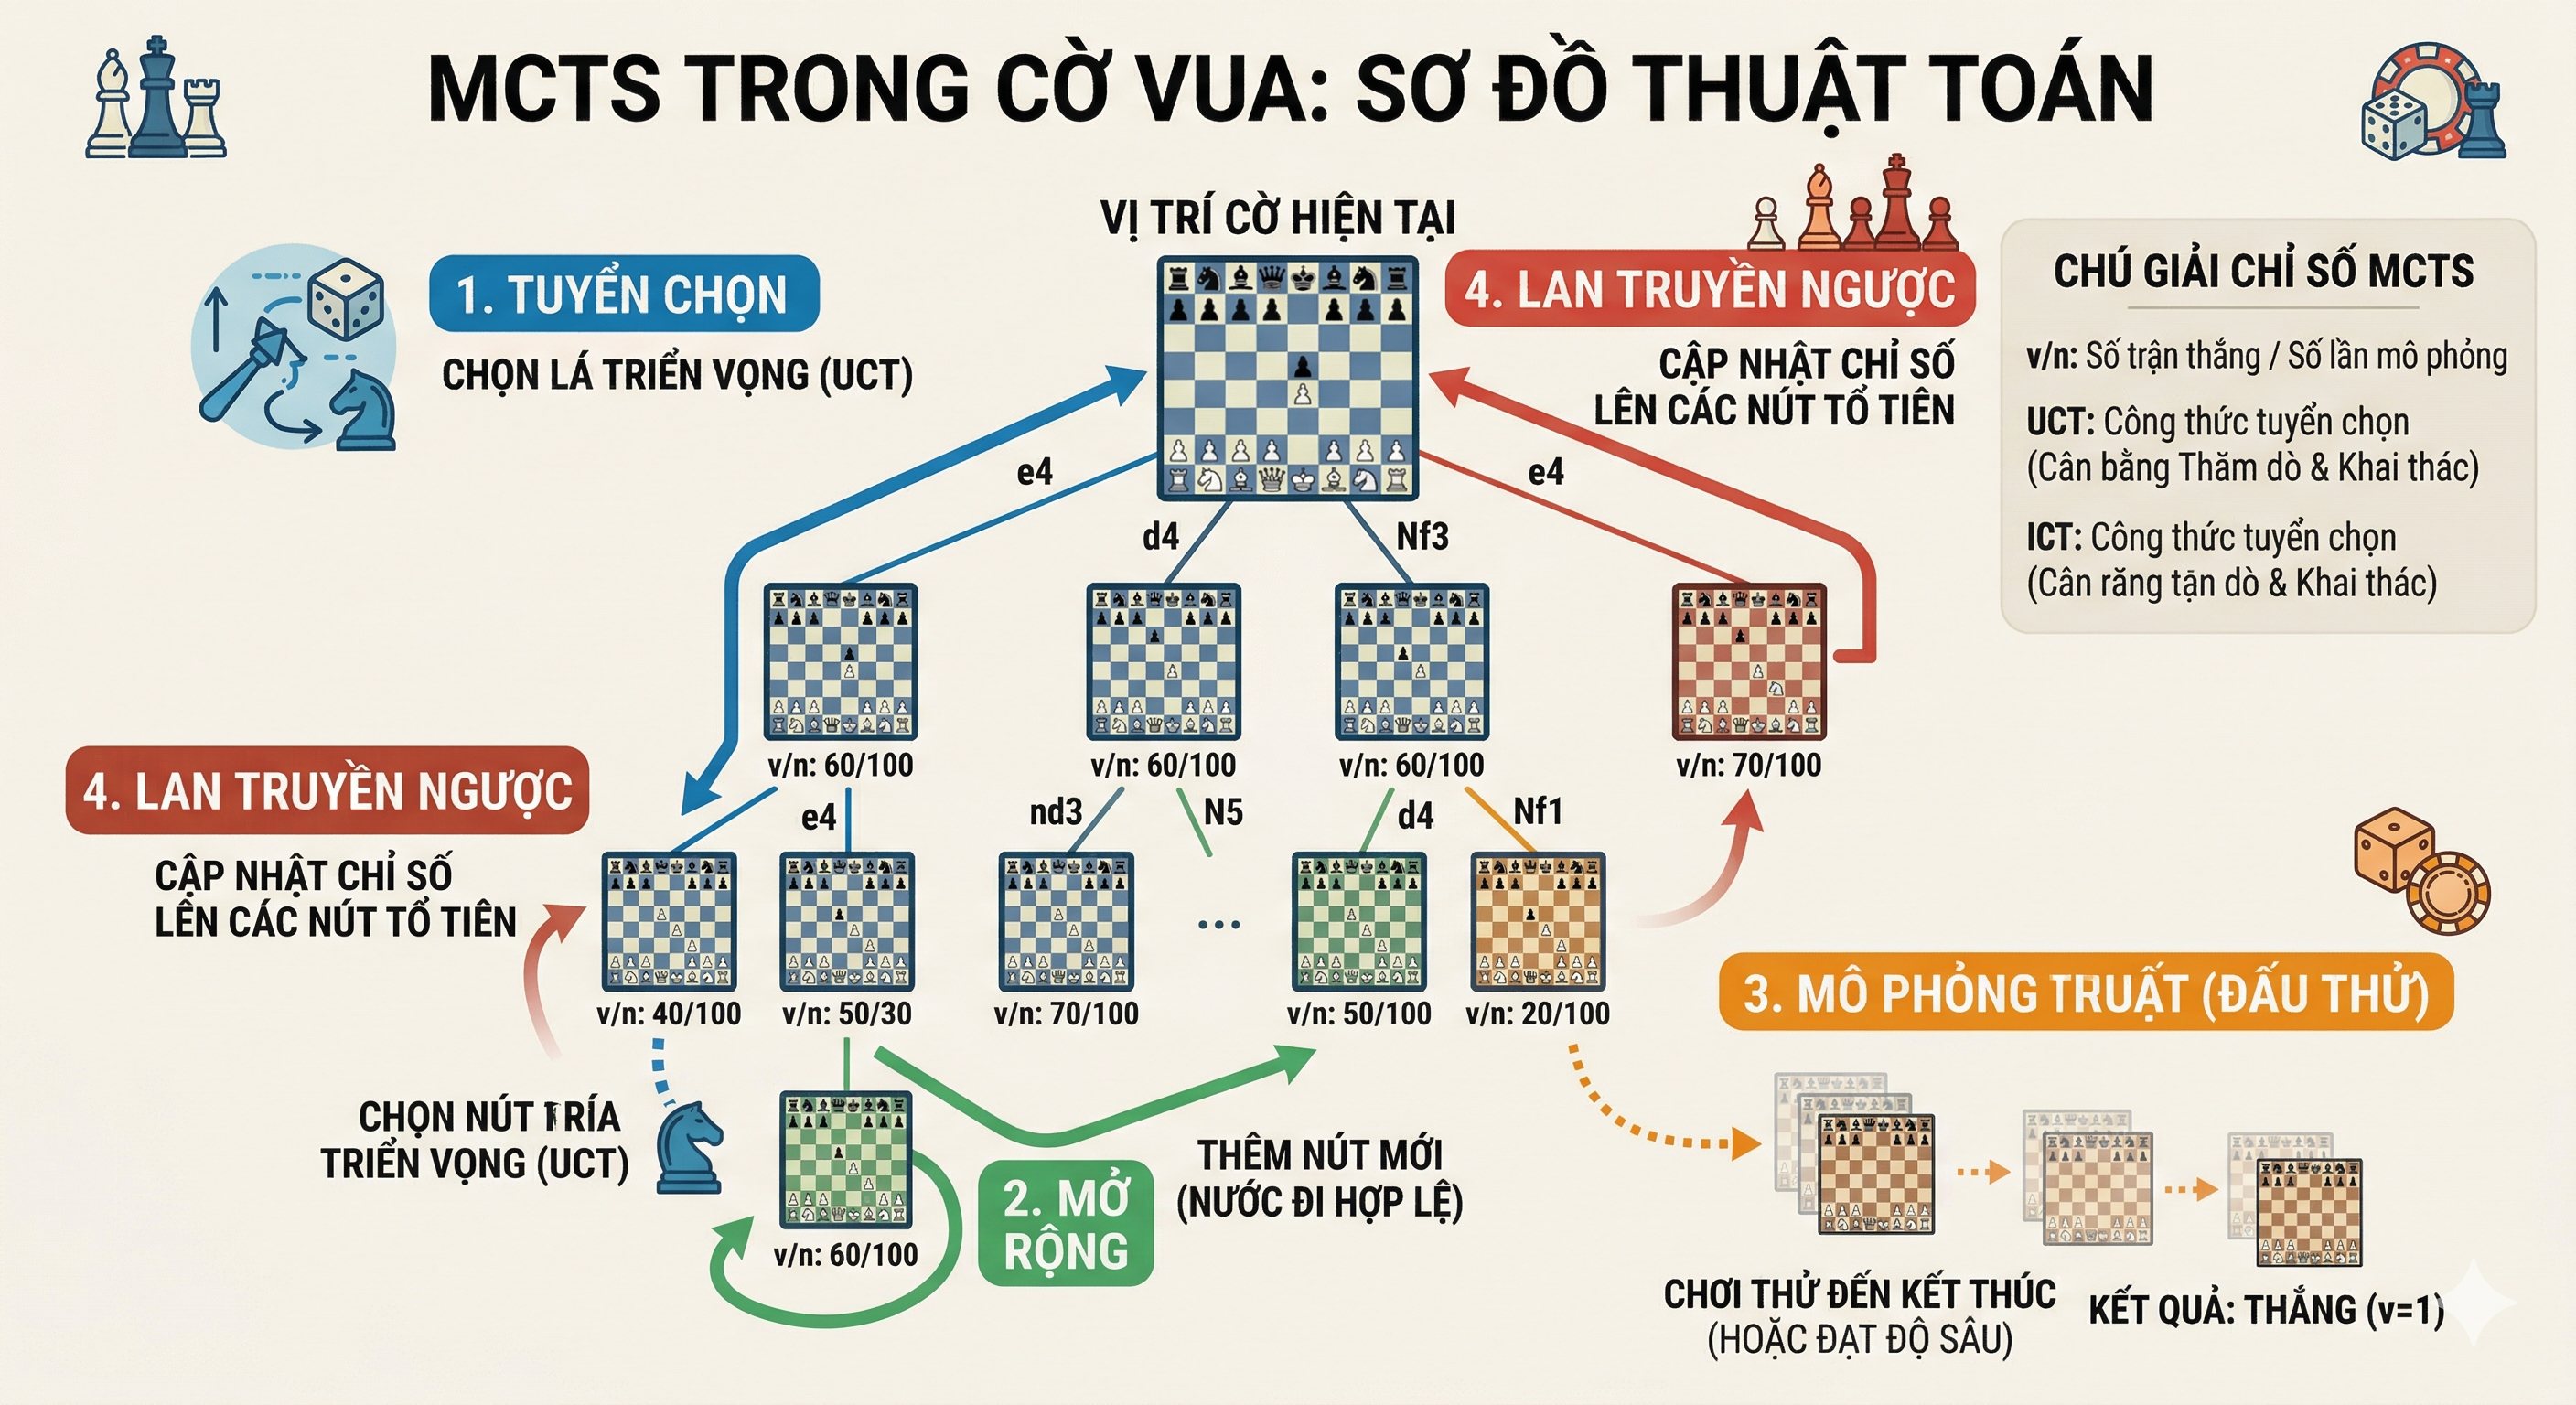
\includegraphics[width=0.8\linewidth]{../../images/ai/illustration-mcts.png}
    \caption{Mô phỏng các kịch bản kết thúc ván đấu trong quy trình MCTS}
\end{figure}

MCTS không cố gắng duyệt sâu theo một hướng cố định, mà nó thực hiện hàng ngàn cuộc "mô phỏng" (rollouts) ngẫu nhiên để xem nước đi nào có tỷ lệ thắng cao nhất. Điều này mang lại một góc nhìn AI hiện đại hơn:
\begin{itemize}
    \item \textbf{Khả năng tự học:} AI có thể "hiểu" thế trận thông qua kết quả của các ván đấu thử nghiệm.
    \item \textbf{Cân bằng giữa khai thác và khám phá:} Sử dụng công thức UCB1 để đảm bảo AI không chỉ tập trung vào các nước đi tốt đã biết mà còn dám thử nghiệm các nước đi tiềm năng mới.
\end{itemize}

\section{Mục tiêu so sánh hai trường phái AI}

Việc đặt Alpha-Beta Pruning (Duyệt cây có hệ thống) cạnh MCTS (Mô phỏng xác suất) trong cùng một dự án nhằm mục đích:
\begin{itemize}
    \item Phân tích xem trong điều kiện tài nguyên hạn chế, thuật toán nào sẽ cho nước đi "người" hơn.
    \item Đánh giá sự đánh đổi giữa thời gian tính toán và độ sâu chiến thuật.
    \item Xây dựng một engine cờ vua đa dạng, cho phép người dùng trải nghiệm hai phong cách chơi khác nhau từ AI.
\end{itemize}
